\documentclass[12pt,a4paper]{article}
\usepackage{float}
\usepackage[utf8]{inputenc}
\usepackage[T1]{fontenc}
\usepackage{graphicx}
\usepackage{listings}
\usepackage{xcolor}
\usepackage{geometry}
\usepackage{hyperref}
\geometry{margin=2.5cm}

\lstset{
    basicstyle=\ttfamily\small,
    keywordstyle=\color{blue},
    commentstyle=\color{gray},
    stringstyle=\color{red},
    showstringspaces=false,
    breaklines=true,
    frame=single,
    numbers=left,
    numberstyle=\tiny\color{gray}
}

\title{Neural Network -- Lab Report}
\author{Le Nghiem Thanh Thuy}
\date{}

\begin{document}

\maketitle

\section{Task of the source}

The source build a simple feed-forward neural network from scratch, only use Python standard library (no NumPy, no PyTorch).

The program have to do two things:
\begin{itemize}
    \item Read the network shape from a file \texttt{structure.txt} (number of layers, and number of neurons each layer).
    \item Two way to set the weights and bias:
    \begin{itemize}
        \item Generate random value for weights and bias.
        \item Or read them from file \texttt{parameters.txt}.
    \end{itemize}
    \item After build the network, do a forward pass with a small input and print the output.
\end{itemize}

The activation function is sigmoid. The input layer do not have weights, it only pass the input to the next layer.

\section{Source design}

\subsection{Class organization}

The source is split into 3 class, each one in a separate file. The file \texttt{Main.py} is the entry point.

\begin{itemize}
    \item \textbf{Neuron} (\texttt{Neuron.py}): the smallest unit. Each neuron hold a list of weights and one bias. It can initialize itself with random value, or set weights and bias from outside. The method \texttt{activate(inputs)} compute the weighted sum and apply sigmoid.
    \item \textbf{Layer} (\texttt{Layer.py}): a layer is a list of Neuron. When the layer do forward, it ask every neuron inside to activate and collect the output to a list.
    \item \textbf{NeuralNetwork} (\texttt{NeuralNetwork.py}): a list of Layer. This class read the structure file, create the layers, and provide method \texttt{forward}, \texttt{initialize\_random\_weights}, \texttt{load\_parameters\_from\_file}, and \texttt{print\_structure}.
\end{itemize}

The relation is simple: \textbf{NeuralNetwork} owns many \textbf{Layer}, and one \textbf{Layer} owns many \textbf{Neuron}.

\subsection{Flow}

The flow of the program is like this:

\begin{enumerate}
    \item \texttt{Main.py} create a \texttt{NeuralNetwork} object.
    \item Call \texttt{build\_from\_file("structure.txt")} -- read number of layers and size of each layer, then build the \texttt{Layer} objects. The first layer is input layer, so its neurons have \texttt{input\_size = 0}.
    \item Set the parameters by one of two way:
    \begin{itemize}
        \item \texttt{initialize\_random\_weights()} -- random for every neuron except input layer.
        \item \texttt{load\_parameters\_from\_file("parameters.txt")} -- read line by line, two line per neuron (one for weights, one for bias).
    \end{itemize}
    \item Call \texttt{forward(input\_data)} -- the input go through layer by layer (skip the input layer because it have no weights). Each layer return its output list, become the input of the next layer.
    \item Print the final output.
\end{enumerate}

The file \texttt{structure.txt} format: first line is the number of layers, then each next line is the size of one layer. The file \texttt{parameters.txt} format: for every neuron (except input layer), one line of weights separated by comma, and the next line is the bias.

\section{Result}

To test the network, we use it to solve the XOR problem. The network shape in \texttt{structure.txt} is set to 2-2-1 (2 input, 2 hidden, 1 output).

I choose weights and bias by hand so the hidden layer act like OR and NAND, and the output layer act like AND. Then the whole network compute XOR (because XOR = OR AND NAND). The parameters in \texttt{parameters.txt} is:

\begin{verbatim}
20, 20
-10
-20, -20
30
20, 20
-30
\end{verbatim}

I test four input: $(0,0)$, $(0,1)$, $(1,0)$, $(1,1)$. The output is close to 0 for $(0,0)$ and $(1,1)$, and close to 1 for $(0,1)$ and $(1,0)$, which match the XOR truth table.

\begin{figure}[H]
    \centering
    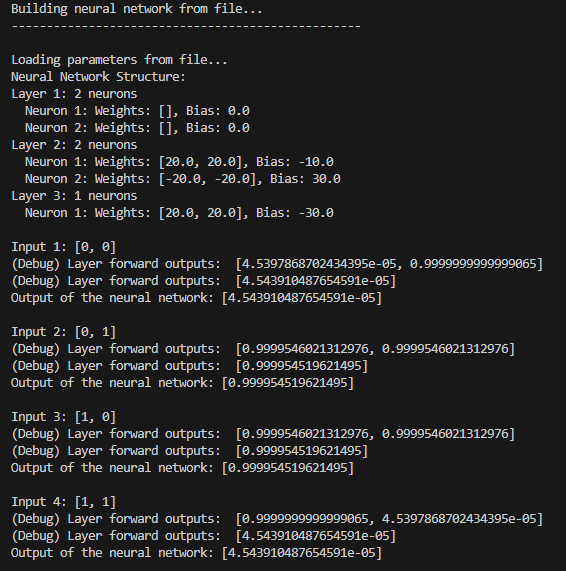
\includegraphics[width=0.9\textwidth]{Result_XOR.png}
    \caption{Output of the network on four XOR input cases.}
    \label{fig:xor}
\end{figure}

\end{document}
